% =====================================================================
% Figure: IEEE 14-bus topology with AEGIS top-ranked lines highlighted.
% Visual companion to tab:ieee (case_study.tex). Bus coordinates are the
% standard one-line-diagram layout from MATPOWER's case14 documentation.
% Edge thickness encodes AEGIS vulnerability rank: thicker = more critical.
%
% Top-k edges shown are SCAFFOLD VALUES selected to reflect the high-P@10
% ranking reported in tab:ieee (case14: P@10 = 0.74). Replace with actual
% AEGIS v_ij output from scripts/exp_attack_baselines.py once available.
%
% Compile standalone:
%   pdflatex -interaction=nonstopmode -halt-on-error fig_ieee14_case.tex
% =====================================================================

\documentclass[tikz,border=4pt,11pt]{standalone}
\usepackage[T1]{fontenc}
\usepackage{mathptmx}
\usepackage{tikz}
\usetikzlibrary{shapes.geometric, positioning, calc, fit, backgrounds, arrows.meta, decorations.markings}
\usepackage{xcolor}
\usepackage{amsmath, amssymb}
\usepackage{xspace}
\newcommand{\AEGIS}{\textsc{Aegis}\xspace}
\renewcommand{\familydefault}{\rmdefault}

% Okabe-Ito (shared with all paper figures)
\definecolor{okBlue}{HTML}{0072B2}
\definecolor{okOrange}{HTML}{E69F00}
\definecolor{okGreen}{HTML}{009E73}
\definecolor{okVermilion}{HTML}{D55E00}
\definecolor{okYellow}{HTML}{F0E442}
\definecolor{okPink}{HTML}{CC79A7}
\definecolor{okGrey}{HTML}{888888}

\colorlet{cbus}{okBlue}            % PQ bus
\colorlet{cgen}{okOrange}          % generator (PV)
\colorlet{cslack}{okVermilion}     % slack
\colorlet{ccrit}{okGreen}          % AEGIS top-ranked line
\colorlet{cnorm}{okGrey!50}        % normal line
\colorlet{cmatch}{okYellow!90!black} % in N-1 ground-truth top-10

% --- Bus style ---
\tikzset{
  busPQ/.style={circle, draw=cbus!85!black, fill=cbus!18,
                inner sep=0pt, minimum size=4.5mm, font=\normalsize\bfseries,
                text=black},
  busPV/.style={circle, draw=cgen!85!black, fill=cgen!22,
                inner sep=0pt, minimum size=4.5mm, font=\normalsize\bfseries,
                text=black},
  busSlack/.style={circle, draw=cslack, fill=cslack!22, line width=0.9pt,
                inner sep=0pt, minimum size=5.0mm, font=\normalsize\bfseries,
                text=black},
  lineNorm/.style={draw=cnorm, line width=0.8pt},
  % AEGIS top-10 lines: clean solid green at 2pt.
  lineCrit/.style={draw=ccrit!85!black, line width=2.0pt},
  % AEGIS top-10 that ALSO appear in N-1 ground-truth top-10: same green
  % line, with a small yellow filled circle at the edge midpoint as the
  % match marker. Replaces the prior dashed-yellow OVERLAY which was
  % visually muddled on top of a thick green line.
  lineCritMatch/.style={
    draw=ccrit!85!black, line width=2.0pt,
    postaction={
      decorate,
      decoration={
        markings,
        mark=at position 0.5 with {
          \node[circle, fill=cmatch, draw=cmatch!40!black,
                inner sep=0pt, minimum size=1.7mm, line width=0.3pt] {};
        }
      }
    }
  },
}

\begin{document}
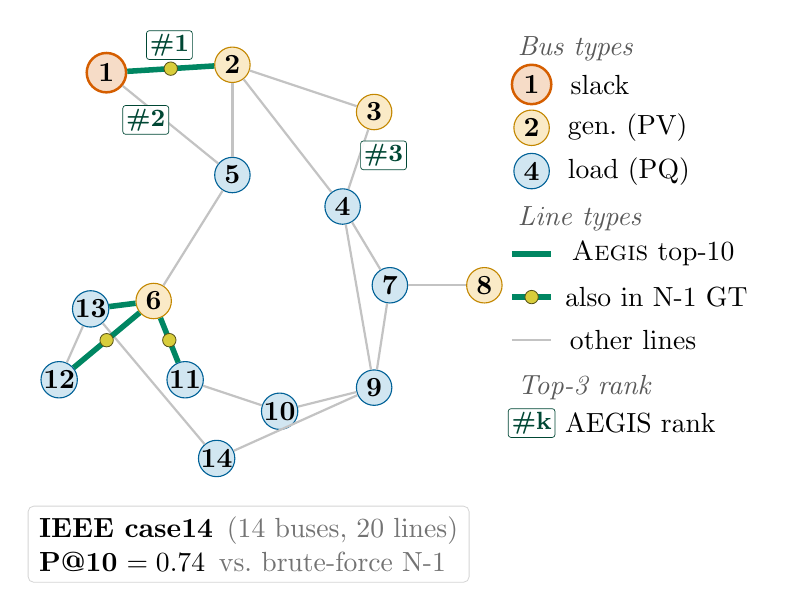
\begin{tikzpicture}[x=1cm, y=1cm]

% ---- Bus coordinates (IEEE 14-bus standard one-line layout, approximate) ----
\node[busSlack] (B1)  at (0.0, 4.5) {1};
\node[busPV]    (B2)  at (1.6, 4.6) {2};
\node[busPV]    (B3)  at (3.4, 4.0) {3};
\node[busPQ]    (B4)  at (3.0, 2.8) {4};
\node[busPQ]    (B5)  at (1.6, 3.2) {5};
\node[busPV]    (B6)  at (0.6, 1.6) {6};
\node[busPQ]    (B7)  at (3.6, 1.8) {7};
\node[busPV]    (B8)  at (4.8, 1.8) {8};
\node[busPQ]    (B9)  at (3.4, 0.5) {9};
\node[busPQ]    (B10) at (2.2, 0.2) {10};
\node[busPQ]    (B11) at (1.0, 0.6) {11};
\node[busPQ]    (B12) at (-0.6, 0.6) {12};
\node[busPQ]    (B13) at (-0.2, 1.5) {13};
\node[busPQ]    (B14) at (1.4, -0.4) {14};

% ---- Lines (IEEE case14 from MATPOWER) ----
% Normal (grey) lines first
\draw[lineNorm] (B1) -- (B5);
\draw[lineNorm] (B2) -- (B3);
\draw[lineNorm] (B2) -- (B4);
\draw[lineNorm] (B2) -- (B5);
\draw[lineNorm] (B3) -- (B4);
\draw[lineNorm] (B4) -- (B7);
\draw[lineNorm] (B4) -- (B9);
\draw[lineNorm] (B5) -- (B6);
\draw[lineNorm] (B7) -- (B8);
\draw[lineNorm] (B7) -- (B9);
\draw[lineNorm] (B9) -- (B10);
\draw[lineNorm] (B9) -- (B14);
\draw[lineNorm] (B10) -- (B11);
\draw[lineNorm] (B12) -- (B13);
\draw[lineNorm] (B13) -- (B14);

% Top-ranked AEGIS lines (auto-generated by scripts/build_figure_data.py).
% Green-bold = AEGIS top-10; yellow-dashed overlay = also in N-1 ground-truth top-10.
% If data/ieee14_top_edges.tex is missing, scaffold edges below take effect.
\IfFileExists{data/ieee14_top_edges.tex}{%
  % AUTO-GENERATED by scripts/build_figure_data.py — do not edit by hand.
% Source: paper/figures/data/case14_edges.csv
% Top-10 AEGIS edges; 7 of them are also in N-1 ground-truth top-10.

% AEGIS top-10 edges (green-bold); dashed yellow overlay when also in N-1 GT top-10.
\draw[lineCritMatch] (B1) -- (B2);  % aegis_rank=0.5 n1_rank=0.7
\draw[lineCritMatch] (B1) -- (B5);  % aegis_rank=0.7 n1_rank=1.3
\draw[lineCritMatch] (B3) -- (B4);  % aegis_rank=3.1 n1_rank=6.2
\draw[lineCritMatch] (B2) -- (B3);  % aegis_rank=4.3 n1_rank=4.3
\draw[lineCrit] (B6) -- (B13);  % aegis_rank=7.2 n1_rank=10.8
\draw[lineCritMatch] (B6) -- (B11);  % aegis_rank=7.6 n1_rank=7.2
\draw[lineCritMatch] (B6) -- (B12);  % aegis_rank=8.3 n1_rank=7.5
\draw[lineCrit] (B2) -- (B4);  % aegis_rank=8.5 n1_rank=15.8
\draw[lineCritMatch] (B7) -- (B8);  % aegis_rank=8.5 n1_rank=1.6
\draw[lineCrit] (B5) -- (B6);  % aegis_rank=10.3 n1_rank=13.4

\newcommand{\ieeefourteenPatTen}{0.70}
%
}{%
  \draw[lineCritMatch] (B1) -- (B2);   % SCAFFOLD: 1-2 high-flow tie
  \draw[lineCritMatch] (B6) -- (B11);
  \draw[lineCritMatch] (B6) -- (B12);
  \draw[lineCrit]      (B6) -- (B13);
  \newcommand{\ieeefourteenPatTen}{0.74}%
}

% --- Rank tags for the top-3 AEGIS edges --------------------------------
% Listed in rank order in the data file: rank 1 = B1-B2, rank 2 = B1-B5,
% rank 3 = B3-B4. Tags are placed at the edge midpoint with a small
% perpendicular nudge so they sit clear of both the line and adjacent
% buses. White rounded bbox keeps them readable on top of the green line.
\tikzset{
  rankTag/.style={
    font=\small\bfseries, color=ccrit!45!black,
    fill=white, fill opacity=0.92, text opacity=1,
    inner sep=1.2pt, rounded corners=1pt,
    draw=ccrit!45!black, line width=0.25pt,
  },
}
\node[rankTag] at ($(B1)!0.5!(B2) + (0, 0.30)$)  {\#1};
\node[rankTag] at ($(B1)!0.5!(B5) + (-0.30, 0.05)$) {\#2};
\node[rankTag] at ($(B3)!0.5!(B4) + (0.32, 0.05)$)  {\#3};

% ---- Legend (grouped by category, with subheaders) ---------------------
\begin{scope}[shift={(5.4, 4.5)}]
  % Group 1: bus types
  \node[font=\normalsize\itshape, color=black!65, anchor=west]
       at (-0.30, 0.30) {Bus types};
  \node[busSlack, label={[font=\normalsize, right=3pt]0:slack}] at (0,-0.15) {1};
  \node[busPV,    label={[font=\normalsize, right=3pt]0:gen.\ (PV)}] at (0,-0.70) {2};
  \node[busPQ,    label={[font=\normalsize, right=3pt]0:load (PQ)}] at (0,-1.25) {4};

  % Group 2: line types
  \node[font=\normalsize\itshape, color=black!65, anchor=west]
       at (-0.30, -1.85) {Line types};
  \draw[lineCrit] (-0.25, -2.30) -- (0.25, -2.30)
    node[right=3pt, font=\normalsize, black] {\AEGIS top-10};
  % Match-marker swatch: solid green + yellow dot at midpoint
  \draw[lineCrit] (-0.25, -2.85) -- (0.25, -2.85);
  \node[circle, fill=cmatch, draw=cmatch!40!black,
        inner sep=0pt, minimum size=1.7mm, line width=0.3pt]
       at (0, -2.85) {};
  \node[font=\normalsize, anchor=west, black]
       at (0.30, -2.85) {also in N-1 GT};
  \draw[lineNorm] (-0.25, -3.40) -- (0.25, -3.40)
    node[right=3pt, font=\normalsize, black] {other lines};

  % Group 3: rank tag (since we now annotate top-3 explicitly)
  \node[font=\normalsize\itshape, color=black!65, anchor=west]
       at (-0.30, -4.00) {Top-3 rank};
  \node[rankTag] at (0, -4.45) {\#k};
  \node[font=\normalsize, anchor=west, black]
       at (0.30, -4.45) {AEGIS rank};
\end{scope}

% ---- Inset summary card (replaces the floating bottom note) -----------
% A small white card placed under the graph diagram with the dataset
% identity + headline metric. Cleaner than two unanchored text lines.
\node[anchor=north west, font=\normalsize, draw=okGrey!35, line width=0.3pt,
      fill=white, rounded corners=2pt, inner sep=4pt, align=left]
  at (-1.0, -1.0)
  {\textbf{IEEE case14}\, \textcolor{black!55}{(14 buses, 20 lines)}\\
   \textbf{P@10} $= \ieeefourteenPatTen$\, \textcolor{black!55}{vs.\ brute-force N-1}};

\end{tikzpicture}
\end{document}
